\documentclass[11pt]{article}
\usepackage{graphicx}
\usepackage{multicol}
\usepackage[total={6.5in,9.0in}, centering]{geometry}
\usepackage{titlesec}
\titleformat*{\subsection}{\small\bfseries}
\usepackage{flexisym}
\usepackage{amssymb}
\usepackage{booktabs}
\usepackage{multirow}
\begin{document}

\begin{multicols}{2}
\section{Algorithm Description}
\subsection{Introduction}
A Binary Search Tree (BST) implements the dictionary abstract data type. In a BST, all the values in a node's left subtree are less than the node value and all the values in the node's right subtree are greater than the node value. Duplicates are not allowed. A BST supports three main operations, viz.: search, insert and delete. Search(\textit{x}) determines if \textit{x} is present in the tree. Insert(\textit{x}) adds key \textit{x} to the tree if it is not already present. Delete(\textit{x}) removes the key \textit{x} from the tree if it is present.

\subsection{Related Work}
Several algorithms have been proposed for non-blocking binary search trees. Ellen[1] and Aravind[2] have proposed a lock-free external BST. An external BST has keys only in the leaf nodes and the internal nodes serve as routing nodes. Howley[3] has proposed a lock-free internal BST. As the tree grows in size, search time dominates and the internal BST tend to perform better than external BSTs as the average path length of an internal BST is half that of an external BST. On the other hand the algorithms described by Ellen[1] and Howley[2] operate on the node level while the algorithm described by Aravind[2] operates on edge level which tend to provide more concurrency when there is high contention. So the algorithm described by Aravind[2] performs well for smaller trees with high contention. We have designed our algorithm to get the benefits of both the worlds. Our algorithm like Howley's[3] is an internal BST and like Aravind's[2] operate on edge level.

\subsection{Overview of the algorithm}
Every operation in our algorithm begins with a seek phase. The operation traverses the search tree from the root node until it finds the target key or it reaches a leaf node. We refer to the path traversed by the operation in the seek phase as the access path. Seek returns references to the last two nodes in the access path. For convenience, we refer to them as parent and node. For insert operation, seek also returns a reference to the injection point where the new node will be inserted. The operation then compares the target key with the value stored in node. Depending on the result of the comparison and the type of the operation, the operation either terminates or moves to the next phase. We now describe the next steps for each of the type of operation one-by-one.

For a \textit{search} operation, if the two keys match, then the operation returns \textit{true} (key was found); otherwise it returns \textit{false} (key was not found).

For an \textit{insert} operation, if the two keys match, then the operation returns \textit{false} (key already exists in the tree); otherwise it moves to the execution phase (key does not exist in the tree). A new node is created and it contains the key being inserted. Finally the insert operation switches the pointer at the node that is pointing to the injection point to point to the new node.

For a \textit{delete} operation, if the two keys do not match, then the operation returns \textit{false} (key does not exist in the tree); otherwise it moves to the execution phase (key does exist in the tree). Delete can be of two types, viz.: simple and complex. Deletion of a node with less than two children is a simple delete and deletion of a node with exactly two children is a complex delete. 

In a simple delete, the pointer at the parent that is pointing to the node being deleted is switched to point to the non-null child of the node being deleted. 

Complex delete has three steps: (i) identifying the successor node, which is the smallest node in the right subtree. (ii) copying the successor's key to the node being deleted and then removal of the  successor by a simple delete and (iii) creating a fresh copy of the node and installing it by switching the pointer from the parent to the node being deleted to point to the fresh copy of the node.

\subsection{Details of the Algorithm}
A tree node in our algorithm consists of three fields: (i) \textit{markAndKey} which contains the key stored in the node, (ii) \textit{child} array, which contains the addresses of the left and right children and (iii) \textit{readyToReplace}, which is a boolean flag used by complex delete operation to indicate if a node can be replaced with a fresh copy of it.
This algorithm like the algorithm described by Aravind[2], operates on edge level. A delete operation obtains ownership of the edges it needs to work on by marking them. To enable marking we steal two bits from the child addresses of a node,(i) \textit{deleteFlag}, to denote if the node is undergoing deletion and (ii) \textit{promoteFlag}, to denote if the node is undergoing promotion. The difference between \textit{deleteFlag} and \textit{promoteFlag} is that \textit{deleteFlag} will be set on the node undergoing deletion while \textit{promoteFlag} will be set on its successor node. A node is said to be marked if any of the \textit{deleteFlag} or \textit{promoteFlag} is set on its child addresses. We also steal another bit (\textit{nullFlag}) from the child address to denote if the corresponding child is null. This serves as a unique null pointer which prevents ABA problem. As complex delete replaces a key in a node being deleted, a flag is required to identify if the key in a node has changed. So we steal a bit from the key field and use it as a mark bit. If the mark bit is set, it denotes that the key in the node has changed.

We next describe the details of the seek phase, which is executed by all operations (search as well as modify) after which we describe the details of the execution phases of insert and delete operations.

\subsection{The Seek Phase}
The seek phase has two steps: traverse step and validation step. In the traverse step an operation traverses the tree along a simple path from the root node to a leaf node, which is referred to as the access path. At each internal node, if the target key is smaller than the node's key it follows the left pointer, if the target key is greater than the node's key it follows the right pointer. If the target key matches the node's key or a leaf node is reached, the traverse step is completed. Also, the seek keeps track of the last unmarked edge in the access path which will be used during helping(explained later). \par
In the validation step the access path is validated. This is required as the key in any node along the access path can change due to a complex delete. In a complex delete we always replace the key in a node undergoing deletion with the smallest key in the right subtree. Hence the value of the key in a node can only increase. This affects the range of keys that can be possibly contained in each of its subtrees. The range in the left subtree expands and the range in the right subtree shrinks. Expanding the range will not affect the seek as the key being searched will still be contained in the subtree. But shrinking the range may require the seek to restart. Like in Howley's[3] algorithm, we keep track of the last edge in which a right path was taken. Once the traverse step is completed, we validate if the key in the last right edge has changed. If yes, we restart the seek, else the seek terminates. \par
An additional validation is required in the seek phase to prevent the below scenario. Consider a tree shown in fig(i) which is being modified by two threads A and B. Assume that thread B starts with delete(\textit{x}). Meanwhile thread A starts seek(\textit{z}) and gets stalled at node \textit{Y} after the right turn it took at node \textit{X}. Now thread B completes delete(\textit{x}) and the tree looks like in fig(ii). Now assume thread B does delete(\textit{w}), which is a complex delete and the key \textit{z} is promoted up the tree and the node \textit{Z} is deleted by a simple delete operation. Now Thread A resumes search(\textit{z}) at node \textit{Y} and finds a \textit{null} node at the left child of node \textit{Y}. It then checks if the key at the last right turn it took at node \textit{X} (which is no longer  a part of the tree) has changed after it had read it. Since it has not changed, search(\textit{z}) terminates and can incorrectly report that \textit{z} is not part of the tree. \par
To avoid this scenario seek keeps track of two seek records, viz.: current seek record and previous seek record. During the validation step, we first check if the key has not changed. If the key has changed we restart the seek phase. If the key has not changed we check if the last right node is unmarked. If it is unmarked then the seek completes and returns the current seek record to the operation which invoked the seek. If the last right node is marked, then seek returns the previous seek record if the last right turn node matches in both the previous and current seek record. Else the seek restarts. This ensures that the seek is linearized correctly.
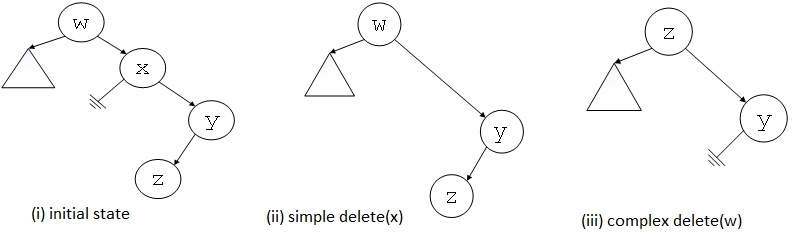
\includegraphics[width=1.0\linewidth]{seek.jpg}

\subsection{Execution Phase of an Insert Operation}
For inserts the algorithms proposed by Ellen[1]and Howley[3] obtain ownership of a node and the algorithm proposed by Aravind[2] obtains ownership of an edge. Our algorithm does not obtain ownership of a node or an edge for an insert operation. Hence in our algorithm an insert operation will not block any other update (insert or delete) operation.\par

Let \textit{key} denote the key to be inserted into the tree and \textit{R} denote the seek record returned by the seek phase. Also let \textit{nKey} denote the key stored in \textit{R$\rightarrow$node}. If \textit{key} matches with \textit{nKey} then \textit{key} is already present in the tree and insert returns \textit{false}. If they do not match a node \textit{newNode} is created and initialized with key \textit{key}. Finally the insert operation tries to replace the edge (\textit{R$\rightarrow$node},\textit{R$\rightarrow$injectionPoint}) with the edge (\textit{R$\rightarrow$node},\textit{R$\rightarrow$newNode}) using a CAS instruction on the appropriate child field of \textit{R$\rightarrow$node}. If the CAS instruction succeeds, then the insert operation has completed. Otherwise, the insert operation performs helping if needed and then retries by re-executing the seek phase. \par
To determine if it needs to perform helping, the insert operation reads the address stored in the child field of \textit{R$\rightarrow$node} on which the CAS failed. If the address is not marked then the injection point has changed due to a successful insert by another thread. So the insert operation of the current thread retries by re-executing the seek phase. If the address is marked then the insert operation has failed due to a concurrent delete operation. If the \textit{deleteFlag} (or \textit{promoteFlag}) is set then it implies that a concurrent delete operation is trying to remove (or promote) \textit{R$\rightarrow$node}. In this case, the insert operation performs helping along the last unmarked edge (\textit{R$\rightarrow$lastUParent},\textit{R$\rightarrow$lastUNode}).\par
To summarize, the execution of an insert operation consists of an alternating sequence of seek and execution phases until the operation terminates. The pseudocode of the execution phase of an insert operation is given in lines 36-47. The steps for creating and installing a new node are given in lines 36-43. In case the CAS instruction fails, the steps for helping a delete operation are given in lines 45-47. Helping, if needed, is performed by invoking a deepHelp routine, which is given in lines 278-300.

\subsection{Execution Phase of a Delete Operation}
Let \textit{R} denote the seek record returned by the seek phase. The execution phase of a delete operation may consist of three modes, namely \textit{injection}, \textit{discovery} and \textit{cleanup}. And a delete operation can be of two types, namely \textit{simple} and \textit{complex}. To keep track of the mode and type of the delete operation a state record is maintained. The structure of a state record is given in lines 12-19. It has six fields: (i) \textit{node}, the node undergoing deletion, (ii) \textit{parent}, parent of the node, (iii) \textit{key}, key to be deleted, (iv) \textit{mode}, current mode, (v) \textit{type}, type of delete operation and (vi) \textit{seekRecord}, seek information for the node undergoing deletion or promotion.

In the injection mode, the delete operation tries to set the \textit{deleteFlag} on the left child edge of \textit{R$\rightarrow$node} using a CAS instruction. If the CAS instruction fails, then the delete operation performs helping in the same way as discussed in the case of insert operation by invoking the deepHelp routine if needed after which it retries starting from the seek phase. If the CAS instruction succeeds, then the delete operation gets the ownership of the node and is guaranteed to complete eventually. As the delete operation owns the node now, the \textit{deleteFlag} is set on the right child using a Bit-Test-and-Set (BTS) instruction. Now the delete operation enters the cleanup mode if it is a simple delete or it enters the discovery mode in case of complex delete.

In the cleanup mode, for a simple delete, the delete operation uses a CAS instruction to remove the node from the tree by trying to replace the edge (\textit{R$\rightarrow$parent},\textit{R$\rightarrow$node}) with the edge (\textit{R$\rightarrow$node},\textit{R$\rightarrow$nonNullChild}), where \textit{nonNullChild} is the appropriate non-null child of the node undergoing deletion. If the node undergoing deletion happens to be a leaf node, then a CAS instruction is used to set the \textit{nullFlag} on the the edge (\textit{R$\rightarrow$parent},\textit{R$\rightarrow$node}). By setting only the \textit{nullFlag} on the edge and not reclaiming the node by setting the edge to \textit{null}, we prevent ABA problem. If the CAS fails, then a concurrent delete operation at the \textit{parent} had prevented the removal of the node. So deepHelp routine is invoked if needed to help finish the pending operation. Then the cleanup of the current delete operation is retried. If the CAS succeeds, then the delete operation is completed. The steps for cleanup for a simple delete are given in lines 233-240.

For a complex delete, an additional step to find and remove the successor node has to be done. So there is a \textit{discovery} mode before the \textit{cleanup} mode. There are two states in the \textit{discovery} mode. The first stage, \textit{findAndMarkSuccessor}, is to find and mark the successor for promotion and the second stage, \textit{removeSuccessor} is to remove the successor. We next describe the details of these two stages.

In \textit{findAndMarkSuccessor} stage, a seek is done to identify the successor node. As mentioned earlier, a successor node is the node with the smallest key in the right subtree. Once a successor node is found, the delete operation tries to set the promote flag on its left edge. If the delete operation gets stalled after this step, then for other threads to help complete this operation they need information of the actual node undergoing deletion. Since the successor is the smallest node in the right subtree, its left child will be \textit{null}. So in a single atomic step a CAS operation copies the address of the node undergoing deletion to the left child of the successor node and sets the \textit{promoteFlag} on it. If the CAS instruction succeeded, then the promote operation will complete eventually. Now if the current delete operation gets stalled, any other threads can see a \textit{promoteFlag} on this edge and identify that this node is undergoing promotion and then they can read the address on the left child to identify the actual node under deletion. But if the CAS instruction fails, then a concurrent delete operation is blocking the current delete operation and deepHelp routine is invoked to help finish the concurrent delete operation. Here we need to handle a special case where all the nodes starting from the node undergoing deletion to its successor node are all marked for deletion. If deepHelp routine is invoked here, then a node can try to help itself recursively and end up in a deadlock. To prevent this scenario a special routine named shallowHelp is invoked. This routine overlooks the invariant that a CAS operation has to be done on an unmarked edge and prevents deadlock. Finally if the CAS operation succeeded, the \textit{promoteFlag} is set on the right child using a BTS instruction and the successor's key, with the mark bit set, is copied to the node undergoing deletion.

The \textit{removeSuccessor} stage starts with the following assertions: the delete operation is of complex type, the \textit{deleteFlag} was set on the left and right child of the node undergoing deletion, the successor node has been found and promote flag has been set on its left and right children, the address of the node undergoing deletion is copied to the left child of the successor node and finally the successor key with the mark bit set has been copied to the node undergoing deletion. Let \textit{succNode} denote the successor node and \textit{succParent} denote its parent node. To remove the successor, a CAS instruction tries to replace the edge (\textit{R$\rightarrow$succParent},\textit{R$\rightarrow$succNode}) with the edge (\textit{R$\rightarrow$succParent},\textit{R$\rightarrow$succNode$\rightarrow$rightChild}). CAS also removes the promote flag on the right child. Here we need to take care of a special case where the successor is the immediate right child of the node under deletion. In this case the \textit{succNode} will be the right child of \textit{succParent} and \textit{succParent} is the node under deletion. The \textit{deleteFlag} will be set on the edge (\textit{R$\rightarrow$succParent},\textit{R$\rightarrow$succNode}). So during CAS this \textit{deleteFlag} has to be copied as well. If CAS fails, then shallowHelp or deepHelp routine has to be invoked appropriately as discussed in \textit{findAndMarkSuccessor} stage. After helping the delete operation re-tries to remove the successor. If the CAS is successful, then the \textit{readyToReplace} flag is set on the node undergoing deletion to indicate that the successor node has been removed and the mode is changed to cleanup.

In the cleanup mode, for a complex delete, the delete operation uses a CAS instruction to install a fresh copy of the node. A new node is created. The key from the old node is copied to the new node with the mark bit cleared, the left and right child addresses are copied with the \textit{deleteFlag} bit cleared and the \textit{readyToReplace} flag is cleared as well. Now a CAS instruction tries to replace the edge (\textit{R$\rightarrow$parent},\textit{R$\rightarrow$node}) with the edge (\textit{R$\rightarrow$parent},\textit{R$\rightarrow$newNode}). If CAS fails, then deepHelp routine is invoked to help a concurrent delete operation if needed. Then the cleanup step is retried. If the CAS is successful, then the delete operation is completed.


\subsection{Other Concurrent Binary Search Tree Implementations}

\end{multicols}

\begin{table}[h]
\begin{tabular}{@{}|c|c|c|c|c|@{}}
\toprule
\multirow{2}{*}{\textbf{Algorithm}} & \multicolumn{2}{c|}{\textbf{\begin{tabular}[c]{@{}c@{}}Number of \\ Objects Allocated\end{tabular}}} & \multicolumn{2}{c|}{\textbf{\begin{tabular}[c]{@{}c@{}}Number of Atomic \\ Instructions Executed\end{tabular}}} \\ \cmidrule(l){2-5} 
                                    & \textbf{Insert}                                   & \textbf{Delete}                                  & \textbf{Insert}                                        & \textbf{Delete}                                        \\ \midrule
\textbf{Ellen}                      & 4                                                 & 2                                                & 3                                                      & 4                                                      \\ \midrule
\textbf{Howley}                     & 2                                                 & 1                                                & 3                                                      & upto 9                                                 \\ \midrule
\textbf{Aravind}                    & 2                                                 & 0                                                & 1                                                      & 3                                                      \\ \midrule
\textbf{This work}                  & 1                                                 & 1                                                & 1                                                      & upto 6                                                 \\ \bottomrule
\end{tabular}
\end{table}
\end{document}



















